%%%%%%%%%%%%%%%%%%%%%%%%%
%                          %
% ----- INTRODUCTION ----- %
%                          %
%%%%%%%%%%%%%%%%%%%%%%%%%%

\section{Données de l'étude de Kosinski}

	\subsection{Introduction}

		Michal Kosinski se présente sur son site web\cite{michal-kosinski} comme un "psychologist and data scientist". L'étude qu'il a co-rédigée à l'Université de Stanford en 2016 a eu un impact important sur le monde académique et même industriel, en montrant les possibilités techniques ouvertes par la récolte de données simples d'utilisateurs : les "likes" Facebbok.

		Ainsi, il est montré qu'avec un peu plus de 300 "likes" tirés une personne, il est possible de définir avec une précision remarquable (mieux que son époux/épouse) des traits psychologiques, ainsi que d'autres caractéristiques personnelles.

	\subsection{Résumé}

		Une enquête a été menée auprès d'une population variée de personnes possédant un compte Facebook. Les données concernant leurs "likes" ont été récoltées, ainsi que des données personnelles pouvant être disponible (ou non) selon le souhait de l'utilisateur sur Facebook, comme ses informations démographiques. Des tests psychologiques ont été également réalisés par une certaine partie des utilisateurs afin de pouvoir trouver des corrélations entre les pages likées et certains trraits psychologiques.

		Cette enquête a rencontré un succès très large, et le nombre de personne ayant répondu à l'enquête, au moins en partie, se compte en millions.

		Les résultats présentés à la fin de l'étude sont inattendus : Michal annonce qu'il est possible de prédire certains comportements d'une personne mieux que son entourage le plus proche.

		Un des modèles crées avec les données récoltées, permet d'estimer le profil psychologique d'un participant selon cinq axes différents, en se basant sur ses likes Facebook. La figure~\ref{a-talk1} montre la précision obtenue par le modèle en fonction du nombre de likes utilisé en entrée.

		\begin{figure}[ht]
			\centering
			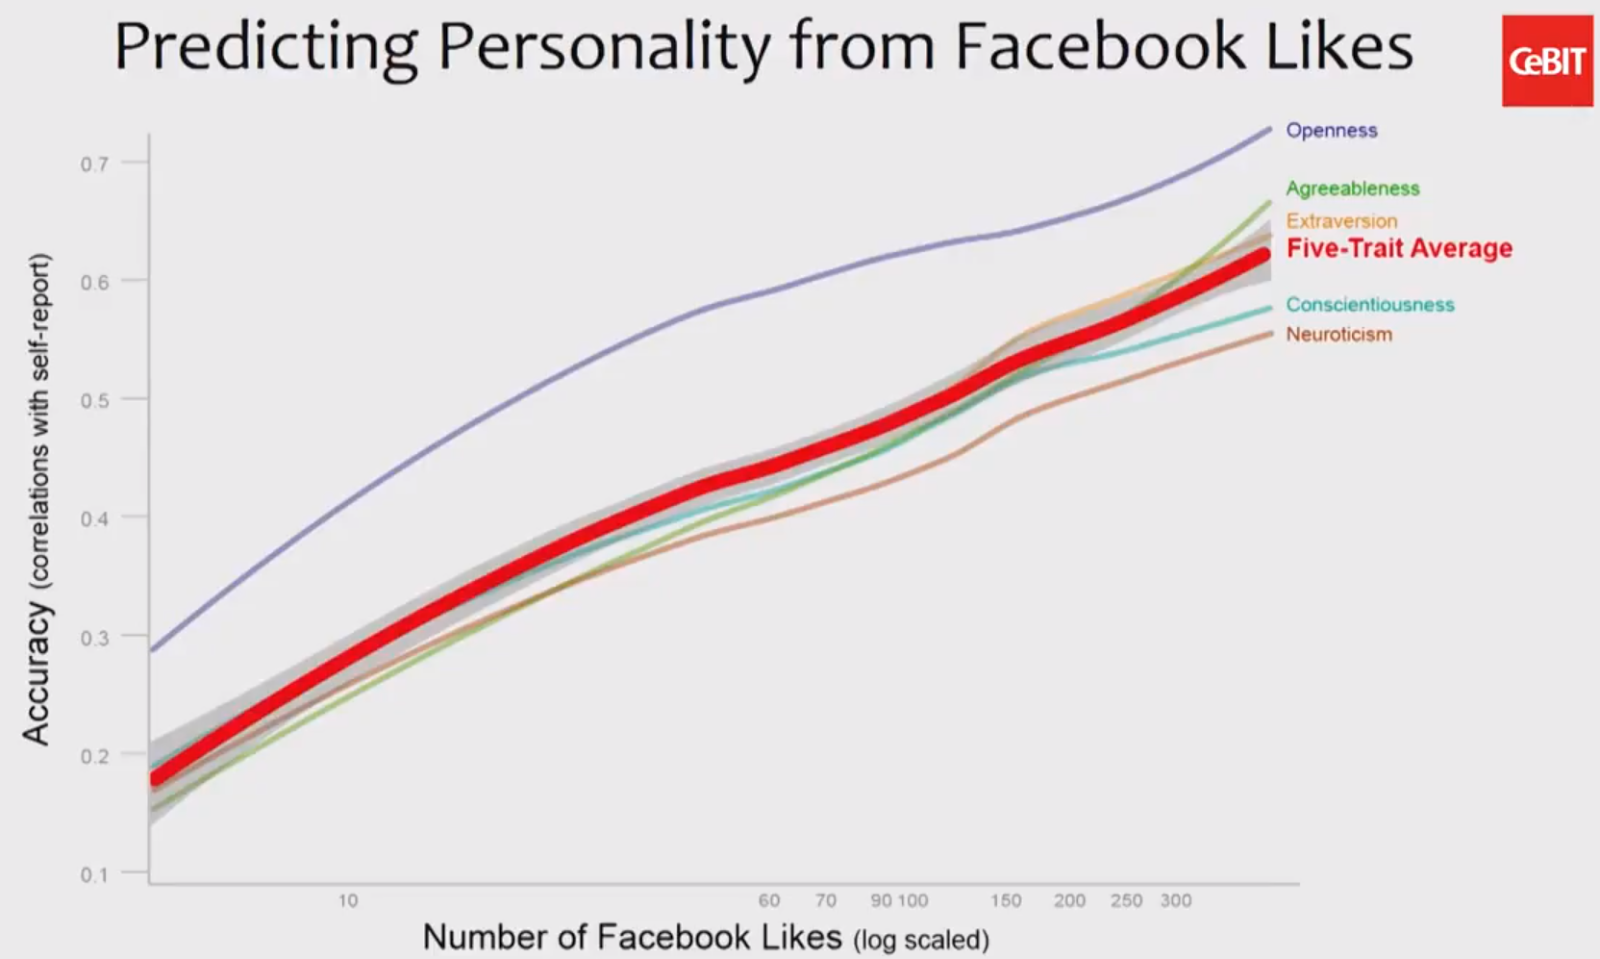
\includegraphics[width=1\textwidth]{images/analysis/talk1}
			\caption{Précision moyenne du modèle prédisant la personnalité d'un utilisateur en fonction du nombre de likes analysés\cite{kosinski-talk}.}
			\label{a-talk1}
		\end{figure}

		On remarque que la précision de la prédiction de tous les critères augmente avec le nombre de likes utilisés, ce qui n'est pas surprenant. En revanche, le tableau~\ref{a-talk-table1} montre le lien entre le nombre de likes utilisés et la précision moyenne atteinte par l'algorithme, et compare ces valeurs à la précision atteinte par d'autres êtres humains.

		\begin{table}[]
			\centering
			\begin{tabular}{lll}
				         & Précision & Nombre de likes \\
				Collègue & 0.27      & 10                            \\
				Ami      & 0.44      & 80                            \\
				Famille  & 0.5       & 100                           \\
				Epoux/se & 0.58      & 250                          
			\end{tabular}
			\caption{Précision atteinte par type de relation avec une personne, et nombre de likes nécessaires au modèle pour égaler sa précision}
			\label{a-talk-table1}
		\end{table}

		On peut voir que la précision de la prédiction de l'algorithme surpasse celle même l'époux/se d'une personne avec 250 likes, ce qui se trouve être légèrement au-dessus du nombre de likes moyen par personne, qui est de 227.

		Les possibilités de prédiction du modèle ne se limitent pas à une simple personne, et les possibilités sont nombreuses. Par exemple, Michal montre qu'il est possible de montrer une corrélation entre les visiteurs d'un certain site web, et une tendance vers certains traits psychologiques. La figure~\ref{a-talk2} montre la personnalité moyenne estimée des visitaurs du site web ```deviantart.com''' par rapport à la moyenne de tous les utilisateurs.

		\begin{figure}[ht]
			\centering
			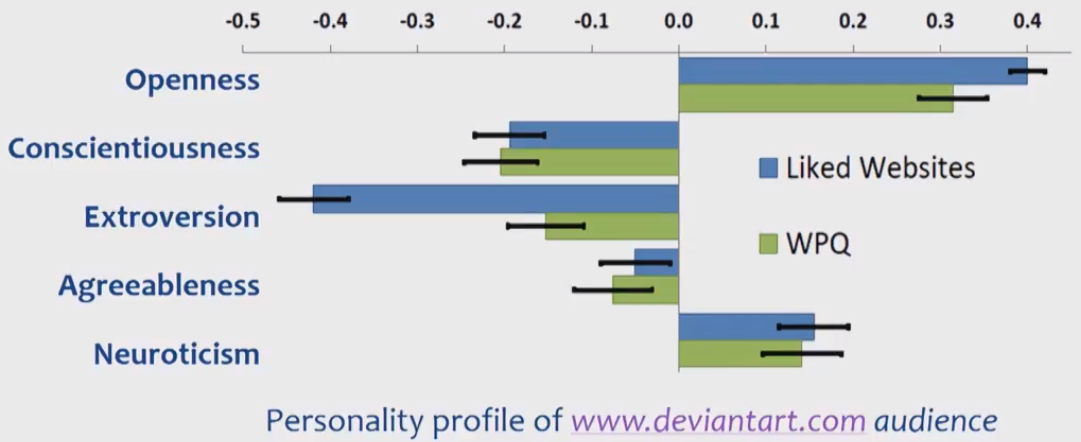
\includegraphics[width=1\textwidth]{images/analysis/talk2}
			\caption{Déviation de la personnalité moyenne estimée d'un visiteur régulier du site ```deviantart.com''' selon les cinq axes psychologiques employés\cite{kosinski-talk}.}
			\label{a-talk2}
		\end{figure}

		Ces corrélations ne sont que quelques exemples parmi un très large éventail de possibles corrélations que le modèle est capable de mettre en lumière. Les implications de telles découvertes sont massives : Il serait par exemple possible de déterminer si un utilisateur sera réceptif ou non à un certain type de publicité, par exemple. Ce genre de problématique touche à plusieurs domaines et n'est pas exactement de notre ressort ici : Des principes éthiques sont en jeu, et le sujet devient de plus en plus délicat. Mais une chose est certaine : Des likes Facebook peuvent révéler énormément d'informations.

	\subsection{Données}

		La quantité de données amassée par l'étude est massive. Non seulement en quantité d'utilisateurs, mais également en diversité de données. Michal Kosinski a mis en place le site web "myPersonnality Project"\cite{mypersonnality} permettant de partager cette source de données avec d'autres chercheurs. Les données comprennent, entre autres :

		\begin{itemize}
			\item Scores de personnalité selon la méthode BIG5 de >3 millions de personnes
			\item Données démographiques de >4 millions de personnes
			\item Localisation géographique de >1.5 million de personnes
			\item Vues politiques de >500'000 personnes
			\item Likes Facebook de >19 millions de personnes
		\end{itemize}

		Le type de données présenté ici n'est qu'un sous-ensemble restreint de l'ensemble des tables présentées, bien qu'il s'agisse ici des données comprenant le plus d'entrées au total.

	\subsection{Acquisition}

		Bien que l'objectif du site web soit de partager l'accès à cette énorme base de données, l'accès à celle-ci est loin d'être aisé. Tout d'abord, Kosinski ne met ces données à disposition que de milieux académiques, il interdit l'utilisation de ces données à des fins commerciales.

		Cependant l'accès n'est pas donné pour autant : Une demande d'accès est à lui envoyer, comprenant une présentation du projet et de ses buts par le biais d'un mail ainsi que le remplissage et l'enregistration du projet de recherche sur des sites spécialisés.

		Cette étape ne semblait constituer qu'une étape nécessiatant un temps restreint, mais un prérequis à l'envoi d'une demande d'accès à la base de données est l'approbation de l'"IRB" (Institutional Review Board), ce qui correspond à un comité d'éthique.

	\subsection{Conclusion}

		Etant donné les délais estimés de l'envoi de la demande à un comité d'éthique responsable puis de la demande d'accès aux données à Kosinski, nous avons écarté cette source de données de la liste principale du projet car nous n'avions pas l'assurance de disposer des données à temps pour la suite de l'étude. Bien qu'il s'agisse certainement d'un ajout conséquent aux données amassées par le projet, nous ne pouvons pas nous permettre de mettre en péril tout l'agenda du projet sur cette source de données.

		Bien que cette base de connaissance ait pu être utile, notre étude va changer de direction. Nous décidons de baser la recherche sur des données que nous récupérerons nous-même.

\section{SDIPI}

	SDIPI signifie "Swiss Digital Identity and Privacy Institute", pouvant se traduire par "Institut Suisse de l'Identité Digitale et de la Vie Privée". Il s'agit d'une association crée dans le but initial de soutenir le projet dans sa visibilité et dans sa légitimité, mais qui aspire à des objectifs généraux plus larges : Le but est de sensibiliser le public Suisse à la manière dont ses informations privées sont  enregistrées, traitées, croisées et utilisées.

	\begin{figure}[h]
		\centering
		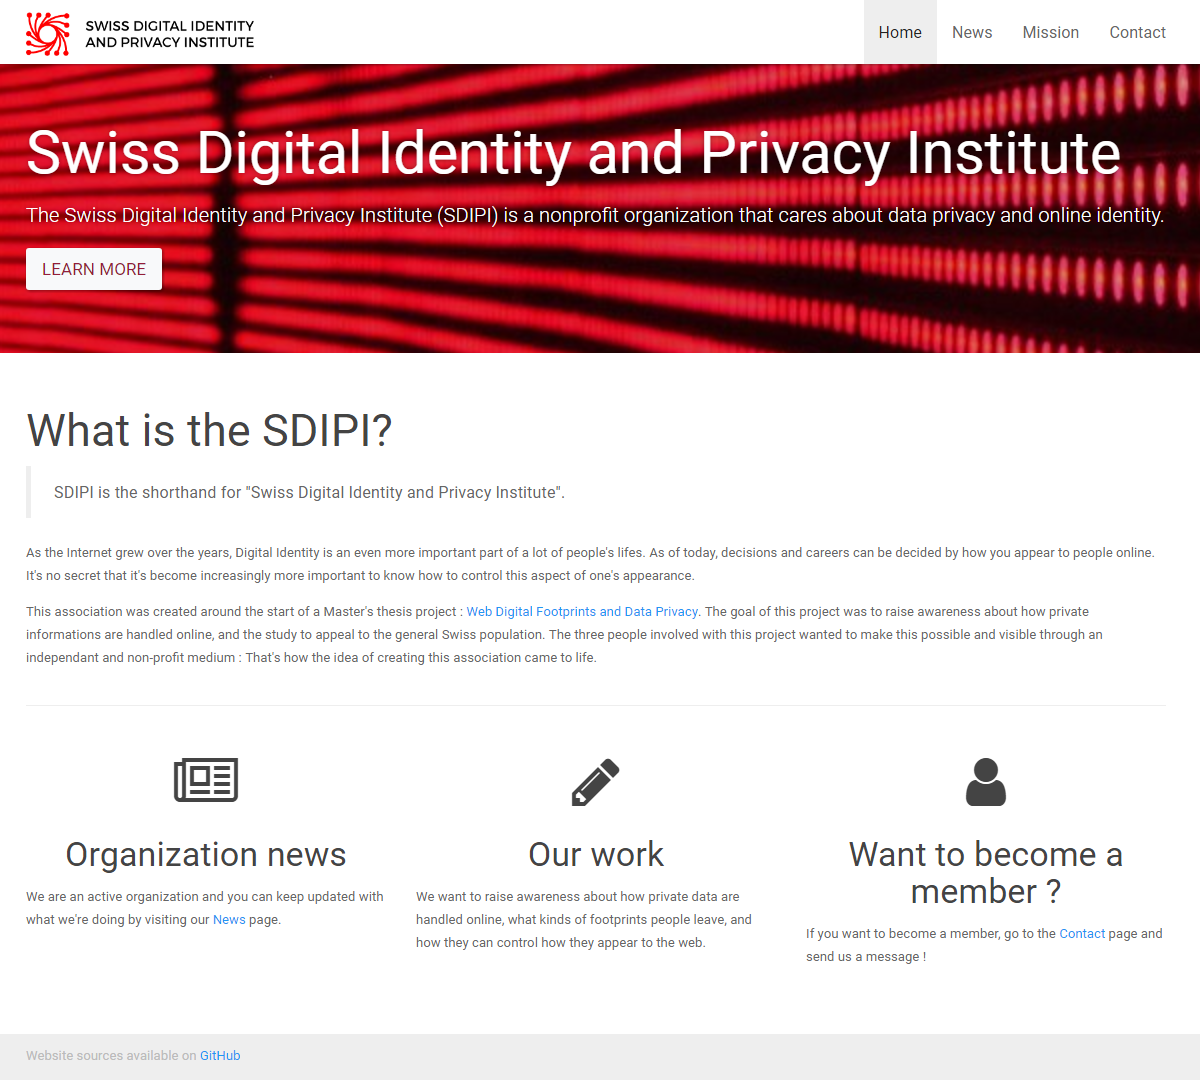
\includegraphics[width=1\textwidth]{images/design/sdipi_home}
		\caption{Page d'accueil du site web \url{https://sdipi.ch}.}
		\label{a-sdipi}
	\end{figure}


\section{Trackers et Google Analytics}

	\subsection{Trackers}

		Un tracker est un serveur contacté lors du chargement d'une page web par un utilisateur. De nos jours, les pages web sont souvent constituées de contenu provenant de plusieurs serveurs ou domaines différents. Il n'est pas rare qu'une seule page web fasse appel à plus d'une dizaine de domaines différents pour charger une seule page. La figure~\ref{a-nbdomains} montre l'évolution du nombre moyen de domaines contactés pour le chargement d'une seule page web, sur les 1'000 sites web les plus visités mondialement.

		\begin{figure}[h]
			\centering
			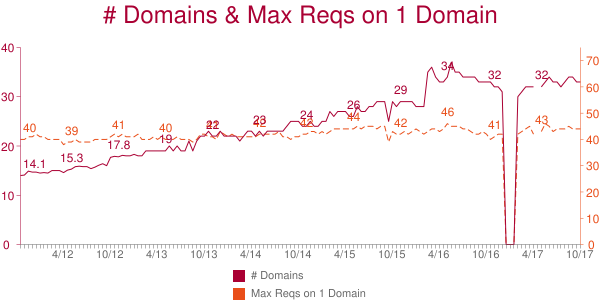
\includegraphics[width=1\textwidth]{images/analysis/nbdomains}
			\caption{Nombre moyen de domaines contactés au chargement d'une page web\cite{nbdomains}.}
			\label{a-nbdomains}
		\end{figure}

		Bien qu'une partie des domaines soient nécessaires à contacter afin de charger du contenu indispensable à la page, une partie d'entre eux ne sert également qu'à des fins statistiques ou publicitaires. Par exemple, ceux-ci peuvent récupérer des informations sur l'utilisateur et son navigateur afin de lui proposer des publicités ciblées sur ses intérêts. Cette pratique est aujourd'hui courante, comme le montre la prochaine sous-section.

	\subsection{Etat de l'art}

		Etant donné que nous nous intéressons aux données des utilisateurs récupérées lors de la navigation Web, nous nous sommes intéressés à connaître quels sont les plus grand trackers sur le web.

		La figure~\ref{analytics-usage} montre la part de marché qu'occupe Google Analytics ainsi que ses compétiteurs sur les sites web Suisses.

		\begin{figure}[!h]
			\centering
			\subfloat[Utilisation de services d'analyse et de tracking\label{a-analytics-usage1}]{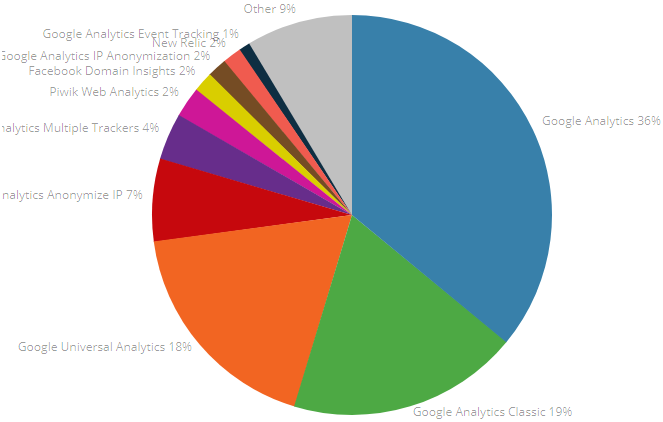
\includegraphics[width=0.45\textwidth,valign=t]{images/analysis/analytics-usage1}}
			\subfloat[Utilisation de services de mesure d'audience\label{a-analytics-usage2}]{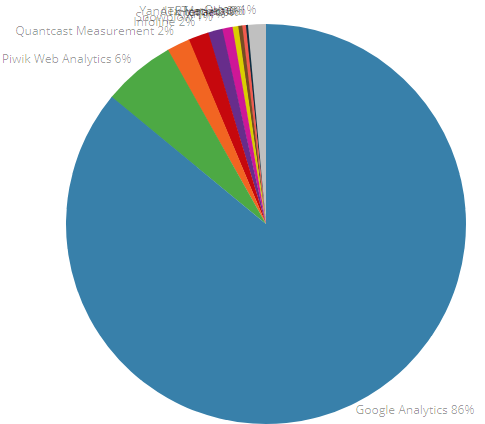
\includegraphics[width=0.45\textwidth,valign=t]{images/analysis/analytics-usage2}}
			\caption{Marché occupé par Google Analytics dans les domaines d'analyse, de tracking et de mesure d'audience sur le Web.}
			\label{analytics-usage}
		\end{figure}

		Nous pouvons calculer grâce au premier graphique que l'ensemble des produits de Google, y compris Google Analytics et ses versions proches, représentent plus de 83\% des installations de solutions dans le domaine de l'analyse et du tracking. De plus pour la sous-catégorie du marché de la mesure d'audience uniquement, Google Analytics a lui seul représente 86\% d'installations sur le Web.

		\begin{figure}[ht]
			\centering
			
\includegraphics[width=0.4\textwidth]{images/analysis/analytics}
			\caption{Logo de la solution Google Analytics\cite{analytics}.}
			\label{a-analytics}
		\end{figure}

		Il est donc de plus en plus évident que s'intéresser aux fonctionnalités de Google Analytics est intéressant pour les buts du projet. Nous souhaitons nous poser la question du risque encouru par les utilisateurs en se connectant sur un site web utilisant Google Analytics. Quelles informations sont prélevées ? Lesquelles sont envoyées ? Les données sont-elles anonymisées ?

	\subsection{Google Analytics}

		Google Analytics se présente comme une solution d'analyse de statistiques d'utilisateurs dans le but d'améliorer les résultats des sites web sur lesquels il est installé. Ce produit étant totalement gratuit pour les PME, il est aujourd'hui très répandu sur le net et particulièrement en Suisse\cite{analytics-usage}.

\section{Extensions de navigateur}

	\subsection{Introduction}

		Au vu de l'objectif du projet qui est à la fois de récolter des données tout en montrant un feedback à l'utilisateur, l'extension pour navigateurs est le moyen le plus facile à la fois pour nous de distribuer notre code, et pour les utilisateurs de l'installer. Cependant, de nombreuxses extensions dont le but est de montrer des statistiques sur la navigation de l'utilisateur existent déjà. L'objectif n'est donc pas seulement d'implémenter les mesures adéquates pour notre étude, mais également de fournir des fonctionnalités à l'utilisateur novatrices afin que l'extension se démarque des concurrents.

		Une analyse des extensions existantes est donc requises afin de prendre des décisions sur la direction que vont prendre les fonctionnalités implémentées.

	\subsection{Etat de l'art}

		Nous nous intéressons aux extensions disponibles pour deux des navigateurs les plus utilisés : Google Chrome, et Mozilla Firefox. Chaque navigateur possède son propre éventail d'extensions, bien que parfois certaines se retrouvent disponibles dans les deux catalogues. Chrome Web Store\cite{chromewebstore} est le catalogue officiel d'extensions pour Google Chrome, et Modules Firefox\cite{modulesfirefox} est celui correspondant à Mozilla Firefox. Quelques recherches avec des mots-clé adaptés sur chaque cataglogue vont nous fournir les extensions les plus populaires pour un thème semblable aux nôtre.

		\subsubsection{timeStats}

			timeStats\cite{timestats} est une extension disponible pour Google Chrome. La figure~\ref{a-timestats} montre comment l'extension se présente via une image montrée sur le Google chrome Store.

			\begin{figure}[h]
				\centering
				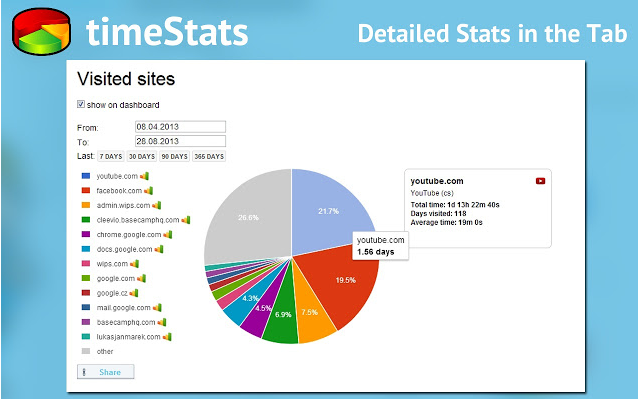
\includegraphics[width=0.6\textwidth]{images/analysis/timestats}
				\caption{Image de présentation de timeStats\cite{timestats}.}
				\label{a-timestats}
			\end{figure}

			Cette extension se focalise sur la visualisation du temps passé sur les différents sites web, parfois regroupés en domaines. La plupart des informations représentées sont le temps passé, et l'extensions s'organise en plusieurs pages permettant de voir des visualisations différentes. On remarque la présence de plusieurs types de graphiques (en ligne, en secteurs) adaptés à la mesure affichée. timeStats est disponible pour Google Chrome uniquement.

		\subsubsection{Ghostery}

			Ghostery est une extension Google Chrome qui possède également sa propre page web en dehors du catalogue. La figure~\ref{a-ghostery} montre la page d'accueil du site ``ghostery.com'', qui est le domaine officiel de l'extension listée sur Google Chrome.

			\begin{figure}[h]
				\centering
				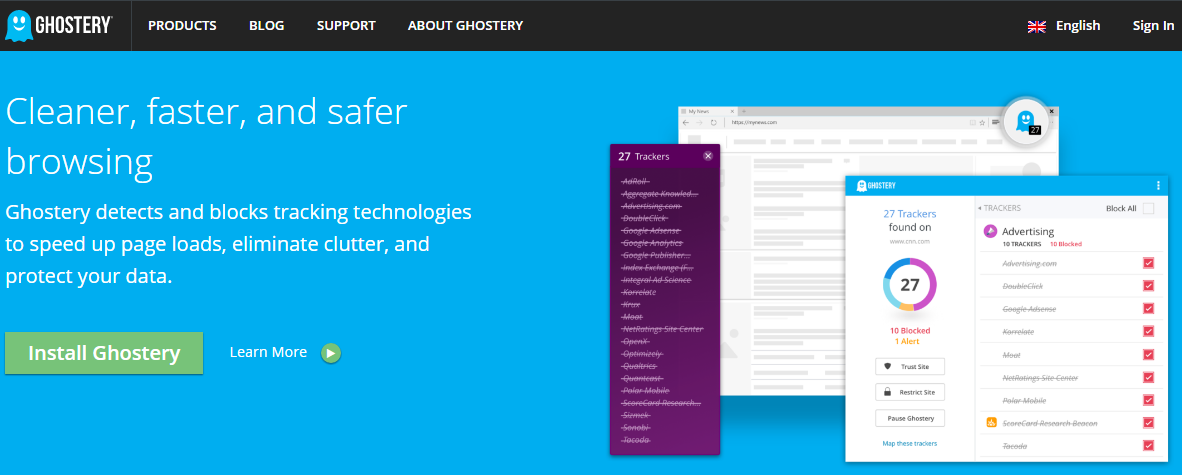
\includegraphics[width=0.8\textwidth]{images/analysis/ghostery}
				\caption{Page d'accueil de Ghostery\cite{ghostery}.}
				\label{a-ghostery}
			\end{figure}

			Ghostery semble donc se concentrer sur la détection et le bloquage des informations envoyées aux trackers tiers lors de la navigation. Quelques options de personnalisation y sont présenter, comme la possibilité d'autoriser des trackers particuliers, ou des domaines choisis.

		\subsubsection{Privacy manager}

			Privacy manager se montre comme une extension permettant la gestion de mécaniques liées à la préservation de la vie privée. La figure~\ref{a-privacymanager} montre l'interface principale utilisée par l'extension.
			Bien que certaines options existent pour la protection de la vie privée, presque la moitié les options activables n'ont pas directement à faire avec la vie privée, et sont plutôt des désactivation ou activations de fonctionnalités de productivité.

			\begin{figure}[h]
				\centering
				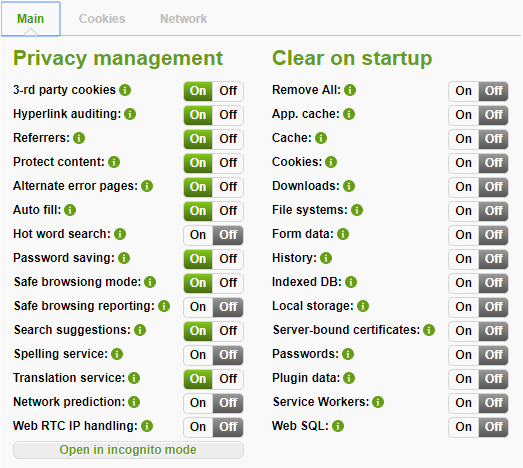
\includegraphics[width=0.5\textwidth]{images/analysis/privacy-manager}
				\caption{Interface de base de Privacy manager\cite{privacymanager}.}
				\label{a-privacymanager}
			\end{figure}

		\subsubsection{TheGoodData}

			TheGoodData remplit à priori la même mission que Ghostery, mais propose des outils légèrement différents, et son thème est centré sur l'utilisation de la valeur des données de navigation pour une bonne cause. Un tableau de bord montré à la figure~\ref{a-thegooddata} permet de se renseigner sur l'état actuel de sa navigation avec des analyses basiques sur les dangers trouvés.

			\begin{figure}[h]
				\centering
				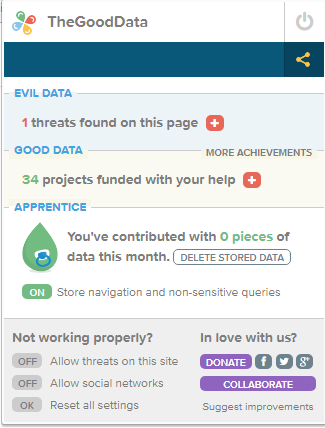
\includegraphics[width=0.4\textwidth]{images/analysis/thegooddata}
				\caption{Interface de TheGoodData\cite{thegooddata}.}
				\label{a-thegooddata}
			\end{figure}

		\subsubsection{Noiszy}

			\begin{figure}[h]
				\centering
				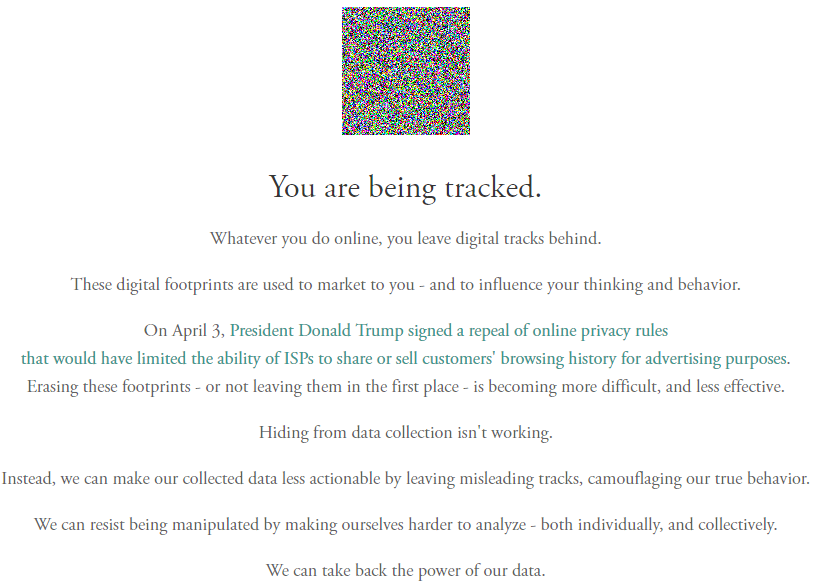
\includegraphics[width=0.9\textwidth]{images/analysis/noiszy}
				\caption{Premier paragraphe de la page web de Noiszy\cite{noiszy}.}
				\label{a-noiszy}
			\end{figure}

			Noiszy cherche quand à lui à brouiller les pistes des trackers existants, sans les bloquer. Son hypothèse de base est qu'il est presque impossible de dissimuler complètement ses "Digital Footprints", et que la meilleure solution est de tenter de les brouiller en les "falsifiant", par exemple en envoyant des données erronnées aux trackers, ou en quantité trop élevées.
			La figure~\ref{a-noiszy} montre le prmier paragraphe de présentation de Noiszy, présent sur leur site web.

		\subsubsection{Privacy Badger}

			Privacy Badger est une extension développée par l'EFF\cite{eff}. Disponible à la fois sur Google Chrome et Mozilla Firefox, cette extension a également comme objectif de contrôler l'envoi de données à des trackers.
			Plutôt que de strictement bloquer toute requête, cette extension laisse à l'utilisateur décider quel niveau de danger représenter chaque tracker, et adapte son comportement entre un bloquage total, la retenue de certaines informations ou aucune action entreprise pour chaque tracker détecté.
			La figure~\ref{a-privacybadger} montre l'interface de l'application une fois celle-ci installée. On peut y voir les lignes de présentant chacune un tracker, et la possibilité de définir son inveau de danger, et par conséquent l'action appropriée associée.

			\begin{figure}[h]
				\centering
				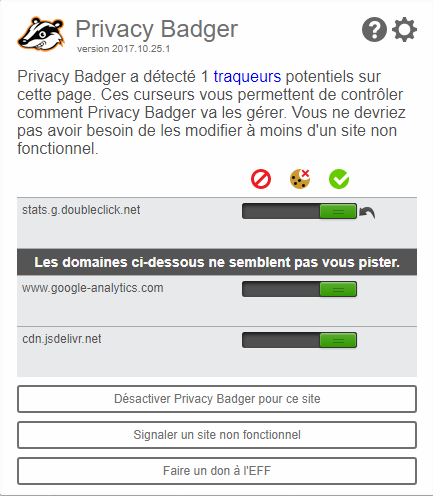
\includegraphics[width=0.5\textwidth]{images/analysis/privacybadger}
				\caption{Contrôle des actions face aux trackers de Privacy Badger\cite{privacybadger}.}
				\label{a-privacybadger}
			\end{figure}

		\subsubsection{Kraken.me}

			Kraken.me est une extension de navigateur, mais également une application pouvant s'installer sur smartphone. Cette application analyse le flux de données de certains services comme Facebook, Twitter, LinkedIn et dencore d'autres. L'objectif est ici de donner à l'utilisateur une vue sur ses propres données, et la manière que celles-si sont utilisées par les applications.
			La figure~\ref{a-krakenme} montre le modèle présenté par le site web.

			Cette application est probablement une des plus semblable à l'objectif général de notre projet, il serait donc intéressant de voir quels ont été les débouchés de cette étude. Notons que la plupart de l'activité de celle-ci ainsi que de l'outil semblent avoir cessé en 2014.

			\begin{figure}[h]
				\centering
				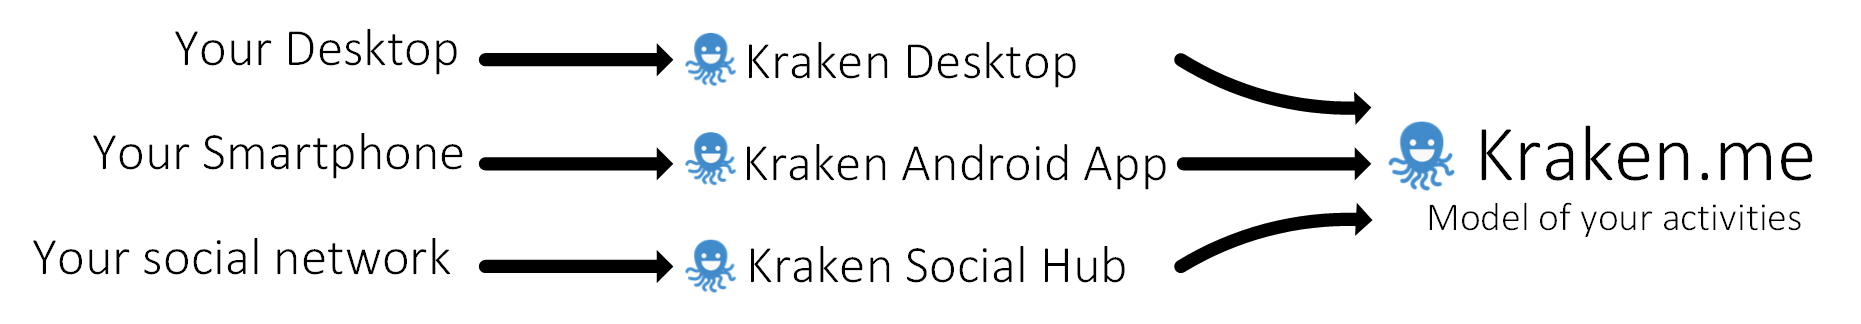
\includegraphics[width=0.8\textwidth]{images/analysis/krakenme}
				\caption{Flux de données de Kraken.me\cite{krakenme}.}
				\label{a-krakenme}
			\end{figure}

	\subsection{Conclusion}

		Après avoir dressé une liste des extensions de navigateur les plus populaires et utilisés, nous pouvons prendre position sur les fonctionnalités que notre extension va posséder afin de se démarquer et de répondre à la problématique de l'étude. Nous allons choisir les fonctionnalités que nous estimons avoir un impact pour la sensibilisation du public aux traces que les internautes laissent, et des informations que nous pouvons en retirer. Ainsi, le plug-in se concentrera sur les deux aspects suivants :

		\begin{itemize}
			\item Détection et mise en lumière des différents trackers présents sur les pages visitées par l'utilisateur.
			\item Tentative de reconstitution du profil de l'utilisateur à partir de la fréquence de la visite des pages web et de leur contenu.
		\end{itemize}
